\documentclass{article}
\usepackage[utf8]{inputenc}
\usepackage{geometry}
\usepackage{graphicx}
\usepackage{listings}
\usepackage{xcolor}
\usepackage{hyperref}
\usepackage{tikz}
\usetikzlibrary{shapes,arrows,positioning}

\geometry{a4paper, margin=1in}

\definecolor{codegreen}{rgb}{0,0.6,0}
\definecolor{codegray}{rgb}{0.5,0.5,0.5}
\definecolor{codepurple}{rgb}{0.58,0,0.82}
\definecolor{backcolour}{rgb}{0.95,0.95,0.92}

\lstdefinestyle{mystyle}{
    backgroundcolor=\color{backcolour},   
    commentstyle=\color{codegreen},
    keywordstyle=\color{magenta},
    numberstyle=\tiny\color{codegray},
    stringstyle=\color{codepurple},
    basicstyle=\ttfamily\footnotesize,
    breakatwhitespace=false,         
    breaklines=true,                 
    captionpos=b,                    
    keepspaces=true,                 
    numbers=left,                    
    numbersep=5pt,                  
    showspaces=false,                
    showstringspaces=false,
    showtabs=false,                  
    tabsize=2
}

\lstset{style=mystyle}

\title{Documentation: Advanced Memory Agent Implementation}
\author{Markdown Knowledge Agent Team}
\date{\today}

\begin{document}

\maketitle

\tableofcontents
\newpage

\section{Introduction}
This document details the implementation of the \textbf{Memory Agent} within the Markdown Knowledge Agent system. The memory module is designed to be an autonomous, active component that intelligently manages conversation history, extracts knowledge, and optimizes context injection for the Large Language Model (LLM).

Unlike simple sliding-window memory systems, this implementation distinguishes between \textit{Passive Memories} (storage mechanisms) and the \textit{Active Agent} (logic for retrieval and management).

\section{Architecture Overview}

The architecture follows a modular design where the \texttt{MemoryModule} acts as the central coordinator.

\begin{itemize}
    \item \textbf{Passive Memories}: Distinct storage backends optimized for different types of data (Semantic, Conceptual, Structural, User Context).
    \item \textbf{Active Agent}: A decision-making layer that determines \textit{what} to recall, \textit{where} to look, and \textit{how} to format the information based on the user's query.
\end{itemize}

\begin{figure}[h]
\centering
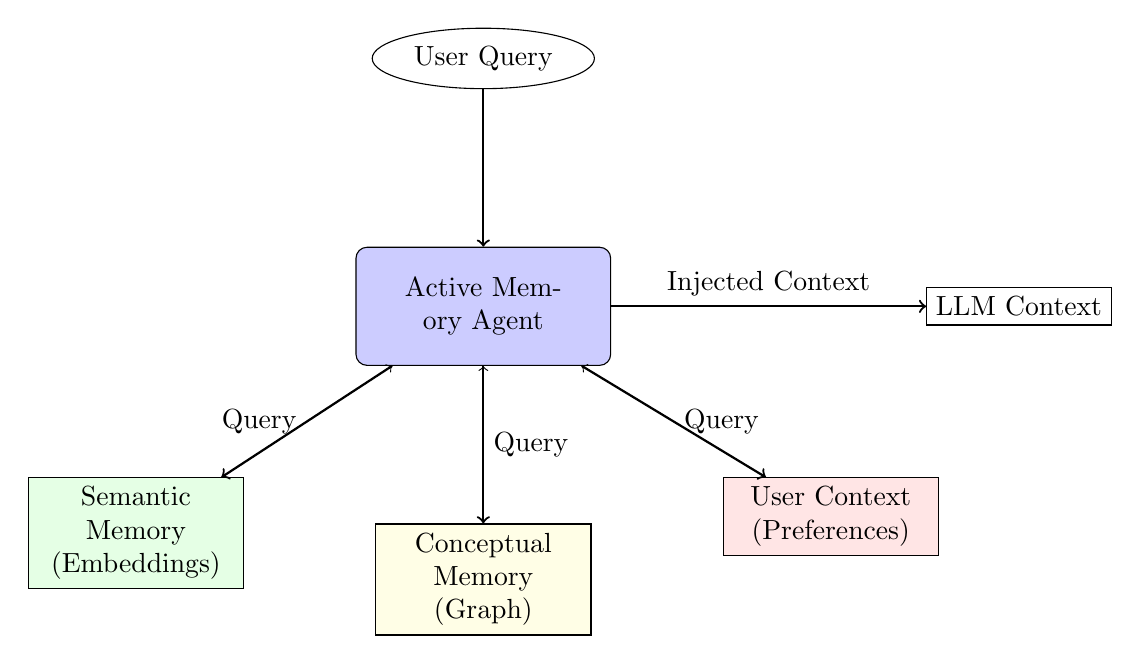
\begin{tikzpicture}[node distance=2cm, auto]
    % Nodes
    \node (agent) [rectangle, draw, fill=blue!20, text width=3cm, text centered, rounded corners, minimum height=1.5cm] {Active Memory Agent};
    
    \node (semantic) [rectangle, draw, fill=green!10, below left=of agent, text width=2.5cm, text centered] {Semantic Memory\\(Embeddings)};
    \node (conceptual) [rectangle, draw, fill=yellow!10, below=of agent, text width=2.5cm, text centered] {Conceptual Memory\\(Graph)};
    \node (context) [rectangle, draw, fill=red!10, below right=of agent, text width=2.5cm, text centered] {User Context\\(Preferences)};
    
    \node (query) [ellipse, draw, above=of agent] {User Query};
    \node (llm) [rectangle, draw, right=of agent, xshift=2cm] {LLM Context};

    % Edges
    \draw[->, thick] (query) -- (agent);
    \draw[->, thick] (agent) -- node[left] {Query} (semantic);
    \draw[->, thick] (agent) -- node {Query} (conceptual);
    \draw[->, thick] (agent) -- node[right] {Query} (context);
    
    \draw[->, dashed] (semantic) -- (agent);
    \draw[->, dashed] (conceptual) -- (agent);
    \draw[->, dashed] (context) -- (agent);
    
    \draw[->, thick] (agent) -- node[above] {Injected Context} (llm);
\end{tikzpicture}
\caption{Memory Agent Architecture}
\end{figure}

\section{Memory Components (Passive Stores)}

\subsection{1. Semantic Memory (Vector Store)}
\begin{itemize}
    \item \textbf{Purpose}: Stores the "meaning" of conversations to allow fuzzy matching and thematic recall.
    \item \textbf{Implementation}: Uses \texttt{sentence-transformers} (model: \textit{all-MiniLM-L6-v2}) to generate 384-dimensional embeddings of user/assistant messages.
    \item \textbf{Storage}: \texttt{faiss} (Facebook AI Similarity Search) index for efficient similarity search ($L2$ distance).
    \item \textbf{Usage}: Retrieved when the user asks "Who", "What", "When", or asks to "remember" something.
\end{itemize}

\subsection{2. Conceptual Memory (Knowledge Graph)}
\begin{itemize}
    \item \textbf{Purpose}: Tracks specific entities, concepts, and keywords mentioned in the conversation.
    \item \textbf{Implementation}: 
        \begin{itemize}
            \item \textbf{Concepts}: Dictionary tracking frequency (\texttt{count}) and first appearance.
            \item \textbf{Index}: Inverted index mapping \texttt{Concept $\rightarrow$ [Message Indices]}.
        \end{itemize}
    \item \textbf{Optimization}: Provides $O(1)$ lookup complexity for keyword-based recall, avoiding full history scans.
\end{itemize}

\subsection{3. User Context Memory}
\begin{itemize}
    \item \textbf{Purpose}: Maintains a persistent profile of the user's interests and preferences.
    \item \textbf{Implementation}: Dictionary tracking domain interest counters (e.g., \texttt{\{"ai": 5, "cooking": 2\}}).
    \item \textbf{Trigger}: Updated when the user expresses preference ("I like...", "I prefer...") or engages deeply with a specific domain.
\end{itemize}

\subsection{4. Short-Term Memory (Buffer)}
\begin{itemize}
    \item \textbf{Purpose}: Maintains immediate conversational continuity.
    \item \textbf{Implementation}: A fixed-size buffer holding the last 4 messages (2 turns).
    \item \textbf{Policy}: Always injected into the context regardless of relevance score.
\end{itemize}

\section{The Active Agent Workflow}

The \texttt{process()} method orchestrates the memory lifecycle for each request:

\subsection{Step 1: Strategy Selection}
The agent analyzes the user's query to decide which memory stores to consult. This prevents unnecessary computation (e.g., not searching vector DB for simple greetings).

\begin{lstlisting}[language=Python]
def _decide_consultation_strategy(self, query: str) -> List[str]:
    strategies = ["short_term"] # Always active
    
    if any(w in query for w in ["who", "what", "remember"]):
        strategies.append("semantic")
        
    if any(w in query for w in ["concept", "summary"]):
        strategies.append("conceptual")
        
    return strategies
\end{lstlisting}

\subsection{Step 2: Consultation \& Retrieval}
The agent executes queries against the selected stores in parallel.
\begin{itemize}
    \item \textbf{Semantic}: \texttt{vector\_index.search(query\_vec, k=3)}
    \item \textbf{Conceptual}: \texttt{concept\_index.get(keyword)}
\end{itemize}

\subsection{Step 3: Ranking and Filtering}
Raw results from different stores are merged. The agent:
\begin{enumerate}
    \item Deduplicates messages (a message might be found by both semantic and conceptual search).
    \item Sorts them chronologically to preserve conversation flow.
    \item Prioritizes Short-Term memory over Long-Term recall.
\end{enumerate}

\section{Optimization Strategies}

\subsection{Token Efficiency}
Instead of sending the entire conversation history (which grows linearly), the agent selects only the most relevant pieces of information.
\begin{itemize}
    \item \textbf{Selective Recall}: Only messages relevant to the current query are retrieved.
    \item \textbf{Result Limit}: Semantic search is limited to top-$k$ results.
\end{itemize}

\subsection{Computational Efficiency}
\begin{itemize}
    \item \textbf{Inverted Indexing}: Conceptual memory uses a hash map for instant lookups, avoiding $O(N)$ string matching across the entire history.
    \item \textbf{FAISS}: Uses optimized C++ bindings for vector similarity search, scalable to thousands of vectors.
\end{itemize}

\section{Visualization}
The system includes a frontend visualization of the \textbf{Knowledge Graph}.
\begin{itemize}
    \item \textbf{Nodes}: Represent concepts (size = frequency).
    \item \textbf{Edges}: Represent co-occurrence of concepts in the same message turn.
\end{itemize}

\end{document}
